
\section{Metodologia}

Foram selecionadas 10 pessoas (tabela \ref{Table-021-ConjuntoIndividuos})
para fazer gravações e nos fonecer dados com a finalidade de estudar o tema e
propor uma rede neural artificial de classificação para identificar os
locutores. Uma vez caracterizada o conjunto de pessoas, a identidade de cada
locutor não é importante. Eles serão, pois, enumerados de 1 a 10.

Um conjunto de 10 frases curtas foram selecionadas para que cada locutor as
proferisse (tabela \ref{Table-022-ConjuntoFrases}), totalizando 100 amostras:
10 indivíduos e 10 frases. Cada frase contém 8 sílabas e o conjunto procurou
explorar diferentes fonemas da Língua Portuguesa.

Com o intuito de aprimorar a capacidade de generalização da rede projetada e de
refletir a impossibilidade de controlar o meio no qual se grava o áudio de
entrada em aplicações reais, 5 ruídos são adicionados às amostras. A base de
amostras contém 600 elementos (equação \ref{Equation-021-AudioDataSet});
portanto.

{
\setlength{\belowdisplayskip}{0pt} \setlength{\belowdisplayshortskip}{0pt}
\setlength{\abovedisplayskip}{0pt} \setlength{\abovedisplayshortskip}{0pt}

\begin{equation}
  m = s + r \times a,
  \label{Equation-021-AudioDataSet}
\end{equation}
}

\noindent onde $s = 100$ é o número de amostras sem adição ruído, $r = 5$ é o
número de elementos da base de ruídos e $m = 600$ é o número total de amostras.
A base final contém 100 amostras sem adição ruído e 500 amostras com adição de
ruído: um total de 600 amostras.

É desejável que o processo de reconhecimento de locutor não dependa do texto
veiculado e, na medida do possível, do tempo de locução. Com a finalidade de
remover os aspectos temporais e extrair parte da informação vocal, aplicamos
transfomadas de Fourier aos sinais de áudio. O algoritmo utilizado foi o
\textit{Fast Fourier Transform} (FFT), variante discreta e eficiente da
transformada de Fourier.

A taxa de amostragem de gravação escolhida foi de 44100 Hz. Essa escolha,
arbitrária, se baseia no fato de que essa taxa de amostragem é a mais comum e
acessível, popularizada por ser a taxa de amostragem utilizada em CDs de áudio.

\begin{center}
  \captionsetup{type=table}
  \begin{tabular}{ c | l | l }
    \textbf{Número} & \textbf{Sexo} & \textbf{Idade} \\
    \hline
     1 & M & 29 \\
     2 & M & 26 \\
     3 & F & 22 \\
     4 & M & 23 \\
     5 & F & 29 \\
     6 & M & 34 \\
     7 & F & 25 \\
     8 & M & 62 \\
     9 & M & 28 \\
    10 & F & 34 \\
  \end{tabular}
  \captionof{table}{
    Conjunto de 10 frases gravadas por cada indivíduo. São frases curtas, de 8
    sílabas, que procuram explorar a riqueza dos fonemas da Língua Portuguesa.
    As gravações foram normalizadas com atenuação de 1 Db. As gravações foram
    editadas para apresentar 2 segundos de duração, cada.
  }
  \label{Table-021-ConjuntoIndividuos}
\end{center}

\begin{center}
  \captionsetup{type=table}
  \begin{tabular}{ c | l }
    \textbf{Número} & \textbf{Frase} \\
    \hline
     1 & Hoje ela mexe muito \\
     2 & Feliz aniversário \\
     3 & Minha mãe gosta de uva \\
     4 & Suco de limão com pera \\
     5 & Minha axila é limpa \\
     6 & Eu tomo chá de gengibre \\
     7 & O treino da rede neural \\
     8 & Envelheço na cidade \\
     9 & Isso é engenharia \\
    10 & Base de frases gravadas \\
  \end{tabular}
  \captionof{table}{
    Conjunto de 10 frases gravadas por cada indivíduo. São frases curtas, de 8
    sílabas, que procuram explorar a riqueza dos fonemas da Língua Portuguesa.
    As gravações foram normalizadas com atenuação de 1 Db. As gravações foram
    editadas para apresentar 2 segundos de duração, cada.
  }
  \label{Table-022-ConjuntoFrases}
\end{center}

\begin{center}
  \captionsetup{type=table}
  \begin{tabular}{ c | l }
    \textbf{Número} & \textbf{Ruído} \\
    \hline
     1 & Trânsito \\
     2 & Escritório \\
     3 & Construção \\
     4 & Chuva \\
     5 & Vento \\
  \end{tabular}
  \captionof{table}{
    Conjunto de 5 ruídos adicionados às gravações. Duração de 2 segundos, cada.
    Sinais de ruído foram normalizados com atenuação em 20 Db --- cerca de 10
    vezes menos intensos do que as gravações.
  }
  \label{Table-023-ConjuntoRuidos}
\end{center}

\begin{figure*}
  \centering
  \captionsetup{type=figure}
  \hspace*{-1.75cm}
  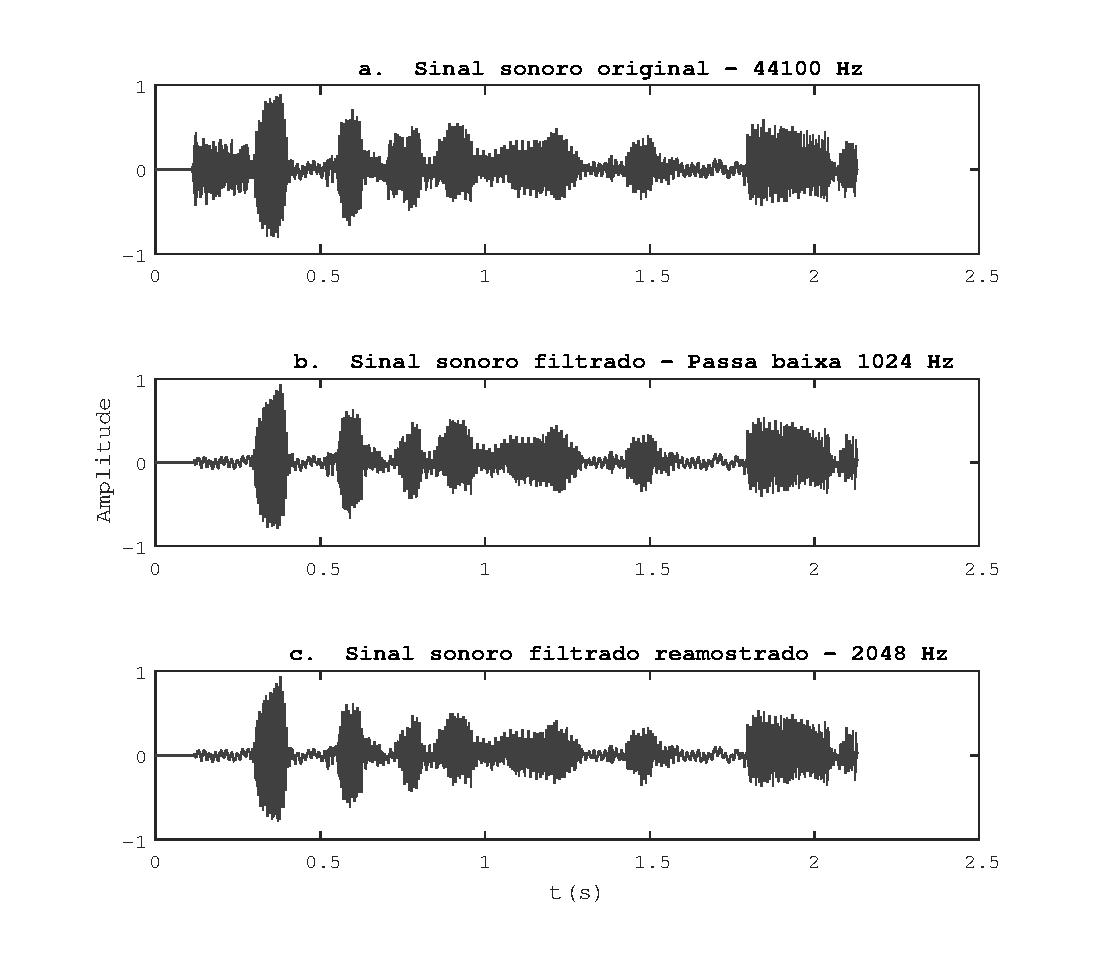
\includegraphics[scale=1]{./figures/Figure-021-SoundSignal.eps}
  \captionof{figure}{
    Manipulações realizadas em um sinal sonoro.\\\\\textbf{a.} $\quad$ Sinal original com
    taxa de amostragem de 44100 Hz.\\\\\textbf{b.} $\quad$Sinal filtrado através de
    Chebshev Tipo II passa baixa [1024; 1152] Hz, com atenuação de 1 Db para
    frequência inferiores a 1024 Hz e atenuação de 60 Db --- atenuação por um
    fator divisor de 1000 --- para frequências acima de 1152 Hz.\\\\\textbf{c.}
    $\quad$ Sinal reamostrado para 2048 Hz.
    \hfill \break
  }
	\label{Figure-021-SoundSignal}
\end{figure*}

\begin{figure*}
  \centering
  \captionsetup{type=figure}
  \hspace*{-1.75cm}
  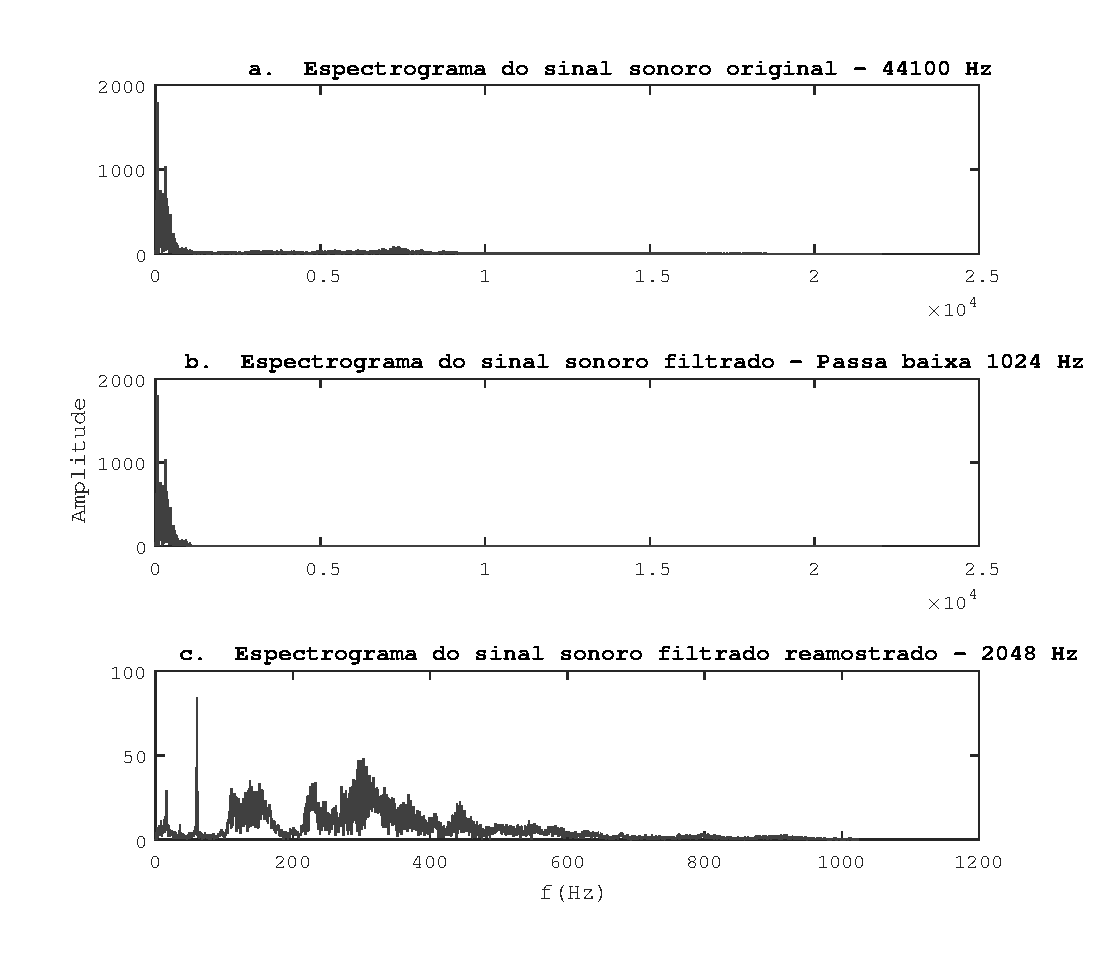
\includegraphics[scale=1]{./figures/Figure-022-Spectrograms.eps}
  \captionof{figure}{
    Espectrogramas dos sinais \textbf{a}, \textbf{b} e \textbf{c} da figura
    \ref{Figure-021-SoundSignal}, respectivamente.
    \hfill \break
  }
	\label{Figure-022-Spectrograms}
\end{figure*}

A taxa de amostragem do sinal nos informa quanto ao número de pontos amostrados
por segundo. O espectrograma resultante da aplicação da transformada de Fourier
contém informação pertinente à metade da taxa de amostragem do sinal --- taxa de
amostragem de Nyquist \cite{Brigham:1988:FFT:83}. Ao aplicarmos a FFT a uma
amostra de áudio amostrado a 44100 Hz (figura \ref{Figure-021-SoundSignal}.a), o
espectrograma resultante (figura \ref{Figure-022-Spectrograms}.a) contém dados
para frequências de até 22050 Hz, inclusive.

Esse espectrograma (figura \ref{Figure-022-Spectrograms}.a) nos
permite avaliar que a maior parte da informação vocal se concentra em baixas
frequências. Para simplificar o modelo contemplado pela rede projetada e remover
ruído do sinal de áudio de entrada, desenvolvemos um filtro passa baixa Chebshev
Tipo II, com frequência de corte de 1024 Hz e atenuação de 60 Db --- o sinal é
atenuado por um fator divisor de 1000. O sinal de áudio filtrado e espectrograma
resultante constam nas figuras \ref{Figure-021-SoundSignal}.b e
\ref{Figure-022-Spectrograms}.b, respectivamente.

Uma vez que o sinal filtrado apresenta pouca ou nenhuma intensidade para
frequências acima de 1024 Hz e preservou parte considerável da informação vocal,
ele foi reamostrado para 2048 Hz. O sinal de áudio filtrado reamostrado e
espectrograma resultante constam nas figuras \ref{Figure-021-SoundSignal}.c e
figura \ref{Figure-022-Spectrograms}.c, respectivamente.

O valor da frequência de corte para filtro passa baixa não foi, de todo,
escolhido arbitrariamente; tampouco a duração do áudio: a aplicação da FFT
apresenta eficiente custo computacional para sequência de dados cujo tamanho
total seja o resultado de uma potência de 2 \cite{Brigham:1988:FFT:131} e
\cite{Brigham:1988:FFT:148}.

O resultado da FFT aplicada ao sinal filtrado e reamostrado é utilizado como
entrada da rede apresentada. Como ele apresenta números complexos, optou-se por
utilizar o valor absoluto de cada ponto, correspondente ao módulo ou magnitude
do mesmo:

{
\setlength{\belowdisplayskip}{0pt} \setlength{\belowdisplayshortskip}{0pt}
\setlength{\abovedisplayskip}{0pt} \setlength{\abovedisplayshortskip}{0pt}

\begin{equation}
  |a + bi| = \sqrt{a^2 + b^2}.
  \label{Equation-021-ComplexModule}
\end{equation}
}

O tamanho final da sequência de entrada para cada amostra da base de gravações é
dado por:

{
\setlength{\belowdisplayskip}{0pt} \setlength{\belowdisplayshortskip}{0pt}
\setlength{\abovedisplayskip}{0pt} \setlength{\abovedisplayshortskip}{0pt}

\begin{equation}
  n = 2048 \times t,
  \label{Equation-022}
\end{equation}
}

onde $t = 2$ segundos é duração de cada amostra, $2048$ é a taxa de amostragem
do sinal de áudio, e $n = 4096$ é o tamanho do vetor de entrada.

A rede proposta é uma rede neural artificial de classificação com camada de
entrada de 4096 pontos, uma camada escondida com 64 neurônios, e camada de saída
com 10 neurônios. Possui função de ativação não linear na camada escondida e
utiliza função de ativação \textit{softmax}. A função de treinamento é a função
do gradiente conjugado escalado.

A matriz de entrada $X_{m\times n}$ possui 600 amostras, cada qual com 4096
pontos, das quais 360 amostras foram utilizadas para treinamento, 120 para
validação e 120 para testes. A partição da amostra é aleatória.

Cada amostra é associada à sua classificação correspondente: um vetor binário
com 10 posições, referentes aos 10 indivíduos --- considerados classes --- onde
o valor 1 na i-ésima posição significa que a amostra pertence à i-ésima classe;
o valor 0, de forma análoga, significa que a amostra não pertence à i-ésima
classe. Cada amostra pertence a uma única classe, naturalmente. Esses vetores
associados às amostras formam a matriz de alvos $T_{m\times c}$, onde $c = 10$ é
o número de classes.

O vetor de saída da rede apresenta, idealmente, as mesmas características de uma
classificação associado a uma amostra.

Na seção 3 são expostos os resultados obtidos pela rede projetada.
